 \begin{savequote}[8cm]
Der Mensch kann tun was er will; er kann aber nicht wollen was er will

Man can do what he wills but he cannot will what he wills.
  \qauthor{--- Arthur Schopenhauer \textit{On The Freedom Of The Will}}
\end{savequote}

\chapter{\label{app:perf}TKI Reconstruction Quality}

\minitoc

\section*{TKI comparisons for the SFGD-$\mu$ sub-sample for the $\numucczpiop$ selection}
\label{sec:app-tki-sfgd-mu}
Figs.~\ref{fig:mc-tki-0pi-esc-sfgmu} and \ref{fig:mc-tki-0pi-mu-sfgmu} provide the response matrix plots and the resolution plots for the $\numucczpiop$ TKI variables of the SFGD-$\mu$ sub-sample respectively.
The comparison is between the performance before the ESC technique and that after the ESC technique, including the Bragg peak cut and the transverse momentum bias correction.
     \begin{figure}
     \centering
          \begin{subfigure}[b]{\dbfigwid\textwidth}
               \centering
               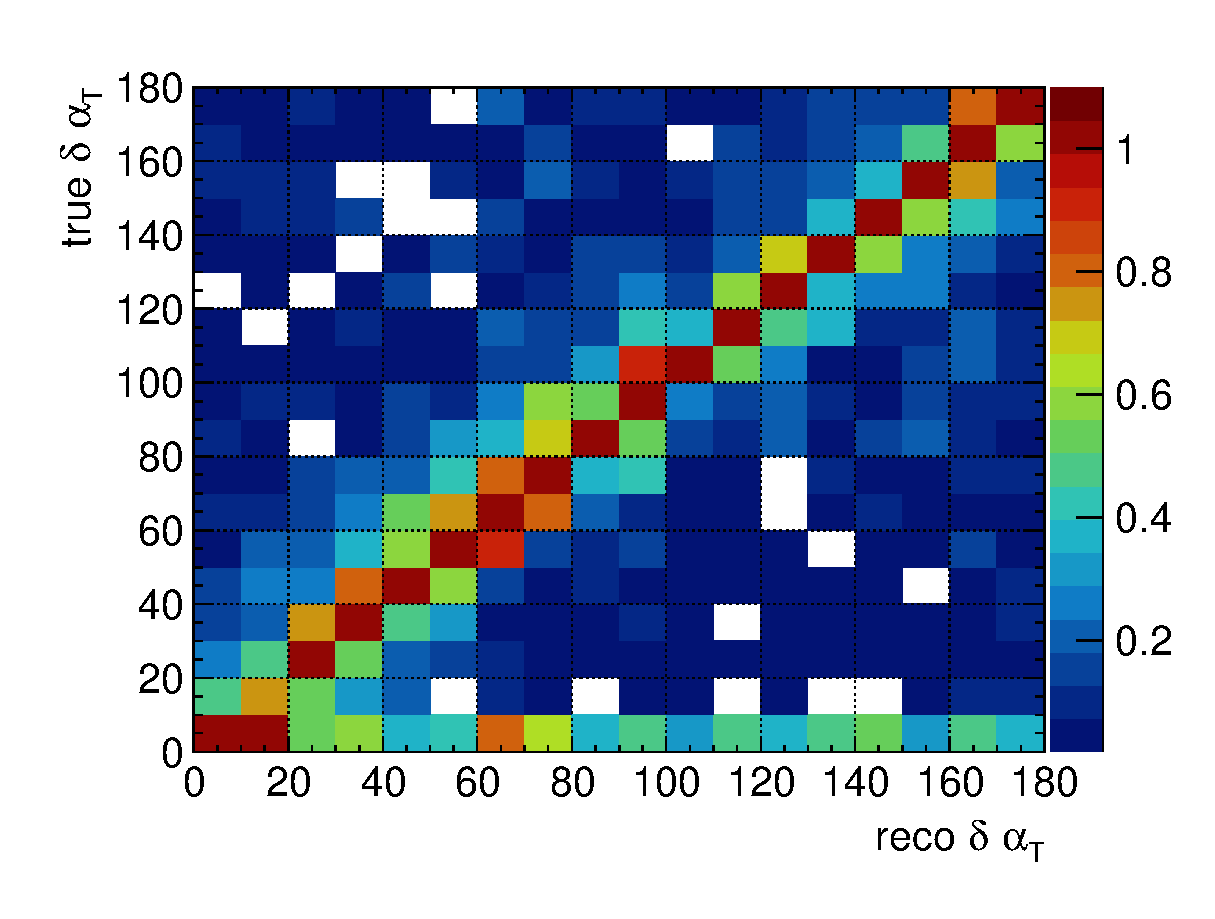
\includegraphics[width=\textwidth]{figures/perf/tki/dalphat_colnor_resmat_al10_sfgmu.eps}
               \caption{$\dat$ before ESC}
               \label{subfig:esc-dalpha-bfesc-sfgmu}
          \end{subfigure}         
          \begin{subfigure}[b]{\dbfigwid\textwidth}
               \centering
               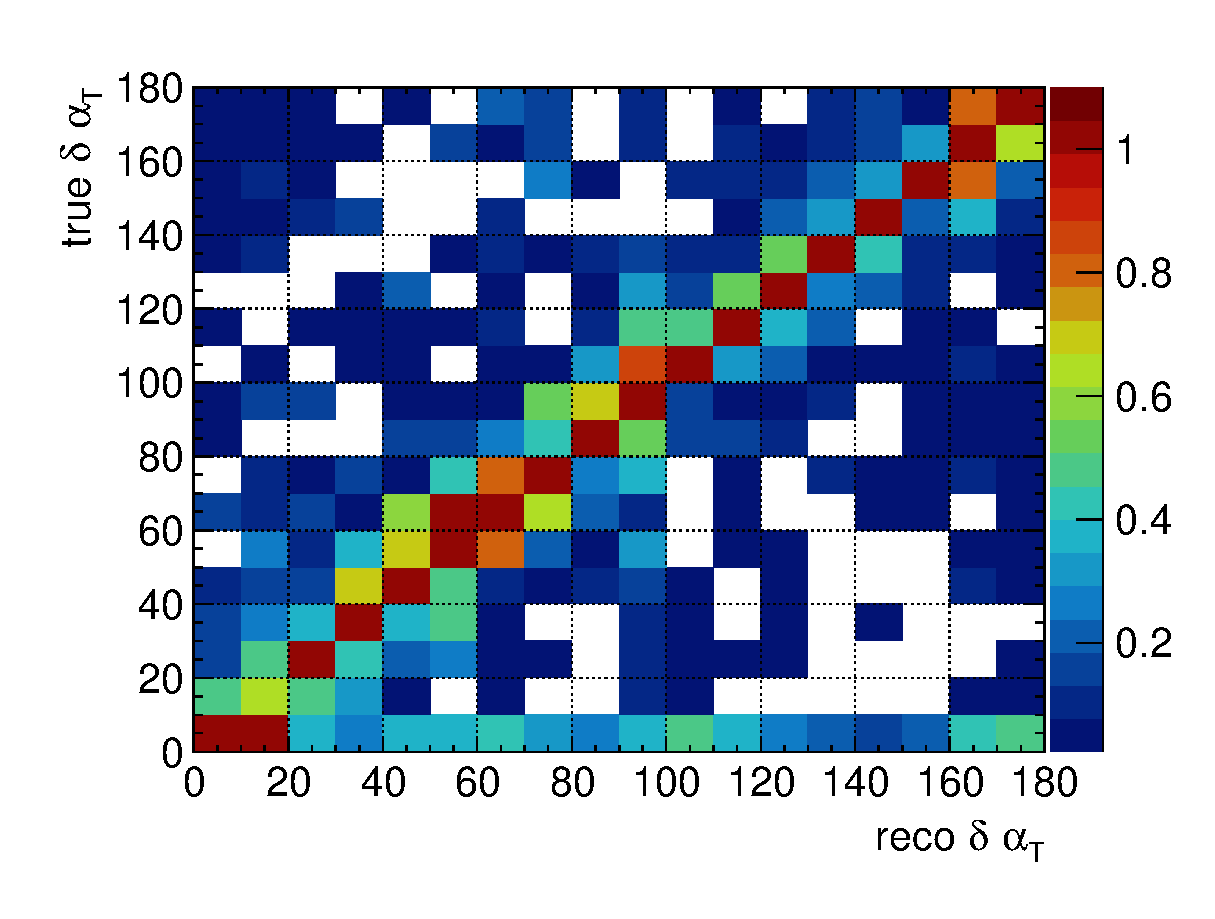
\includegraphics[width=\textwidth]{figures/perf/tki/dalphat_colnor_resmat_al11_sfgmu.eps}
               \caption{$\dat$ after ESC}
               \label{subfig:esc-dalpha-afesc-sfgmu}
          \end{subfigure}
          \\
          \begin{subfigure}[b]{\dbfigwid\textwidth}
               \centering
               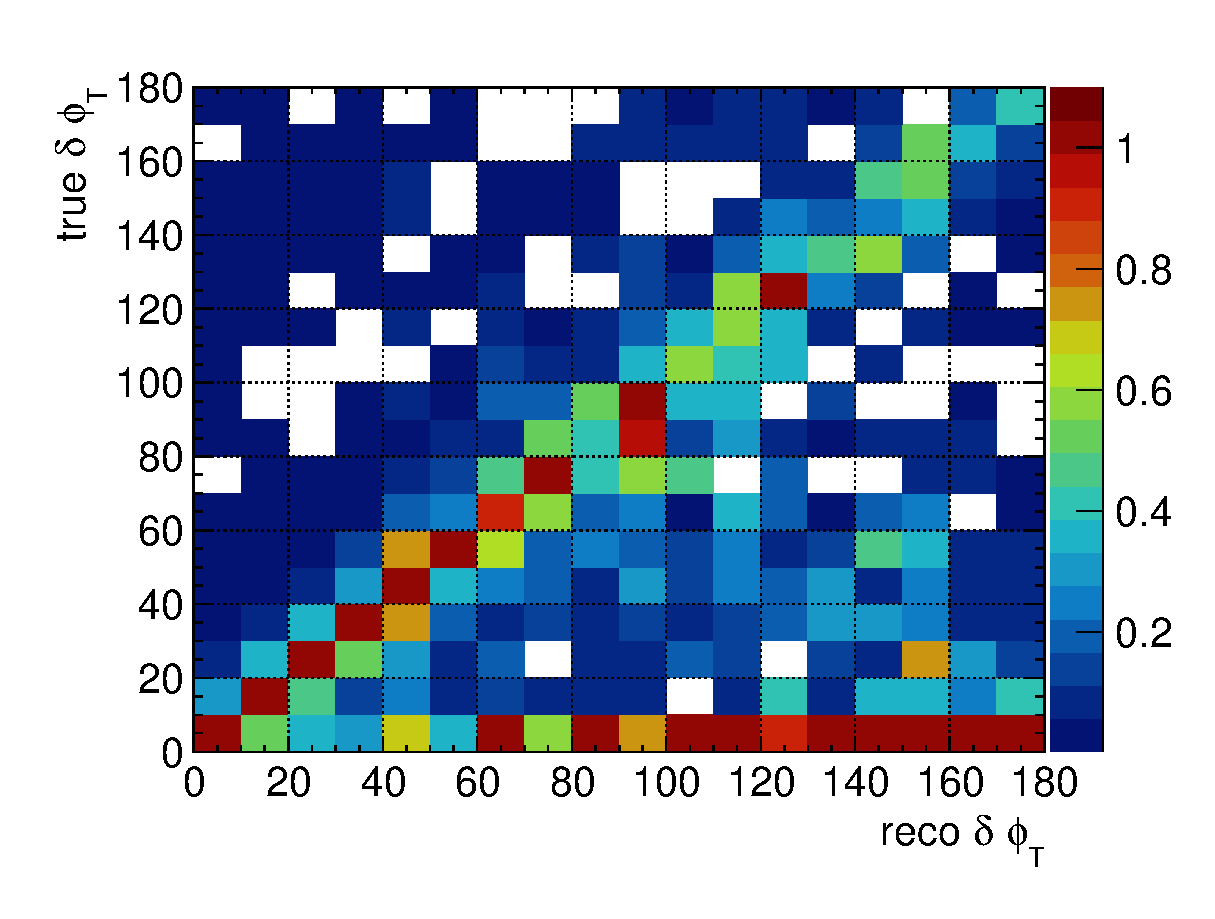
\includegraphics[width=\textwidth]{figures/perf/tki/dphitcolnor_resmat_al10_sfgmu.eps}
               \caption{$\dphit$ before ESC}
               \label{subfig:esc-dphit-bfesc-sfgmu}
          \end{subfigure}
          \begin{subfigure}[b]{\dbfigwid\textwidth}
               \centering
               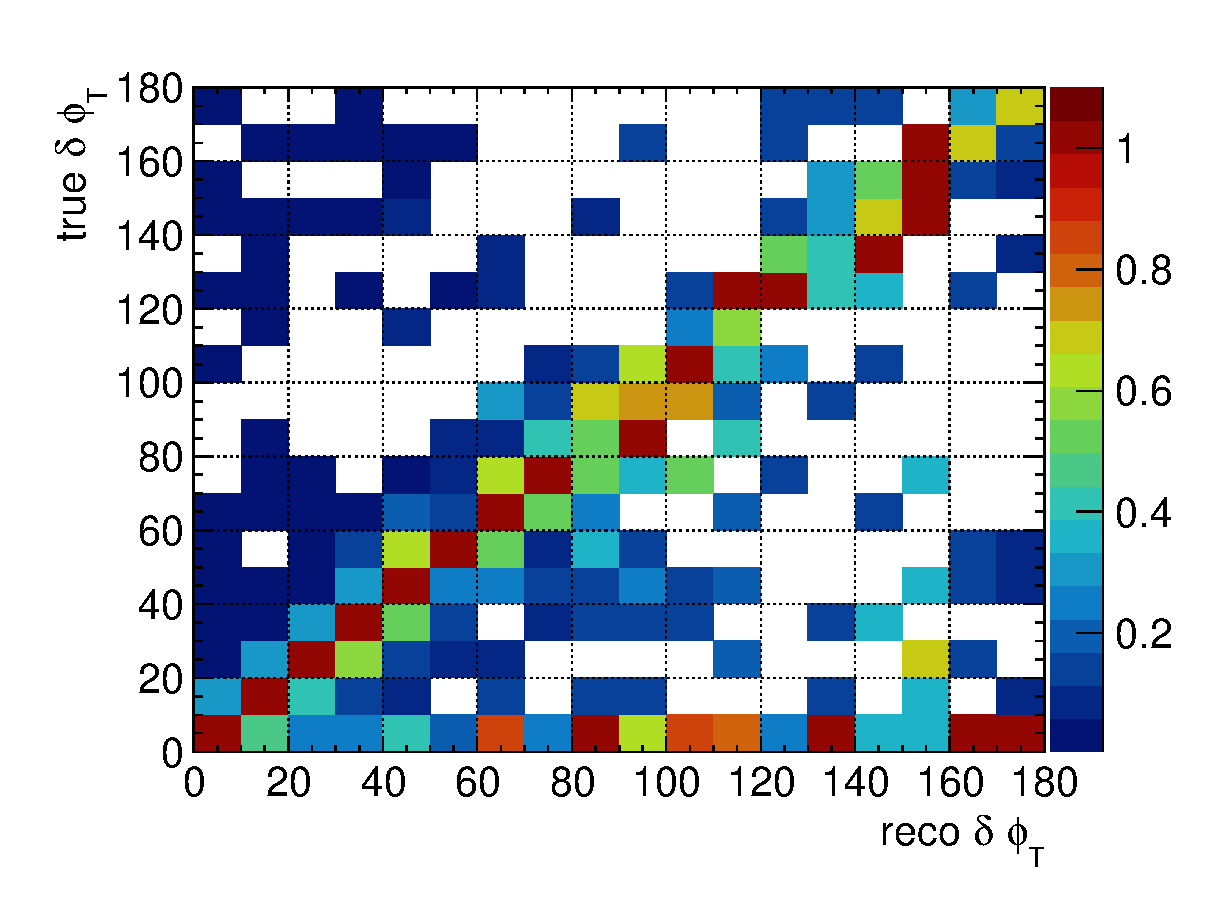
\includegraphics[width=\textwidth]{figures/perf/tki/dphitcolnor_resmat_al11_sfgmu.eps}
               \caption{$\dphit$ after ESC}
               \label{subfig:esc-dphit-afesc-sfgmu}
          \end{subfigure}
          \\
          \begin{subfigure}[b]{\dbfigwid\textwidth}
               \centering
               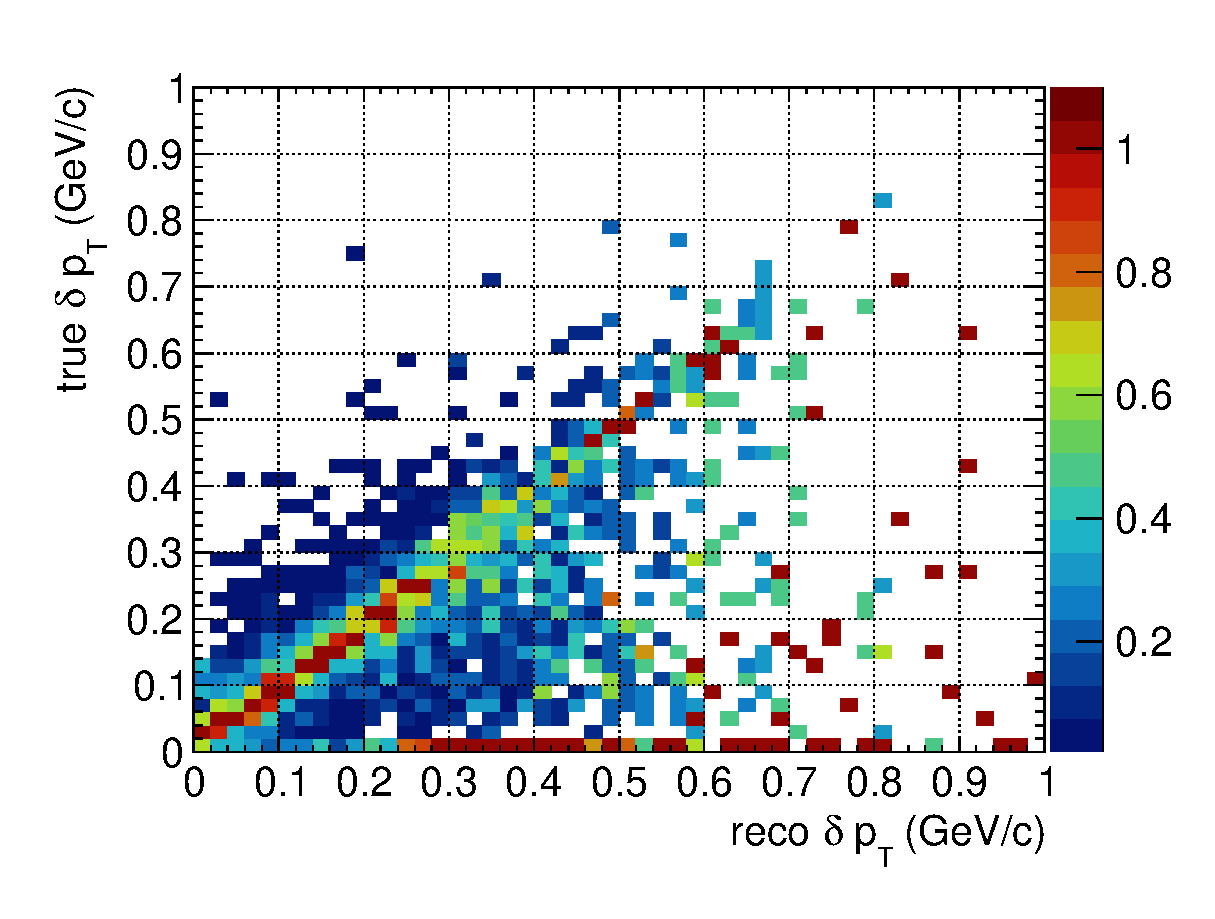
\includegraphics[width=\textwidth]{figures/perf/tki/dpt_colnor_resmat_al10_sfgmu.eps}
               \caption{$\dpt$ before ESC}
               \label{subfig:esc-dpt-bfesc-sfgmu}
          \end{subfigure}
          \begin{subfigure}[b]{\dbfigwid\textwidth}
               \centering
               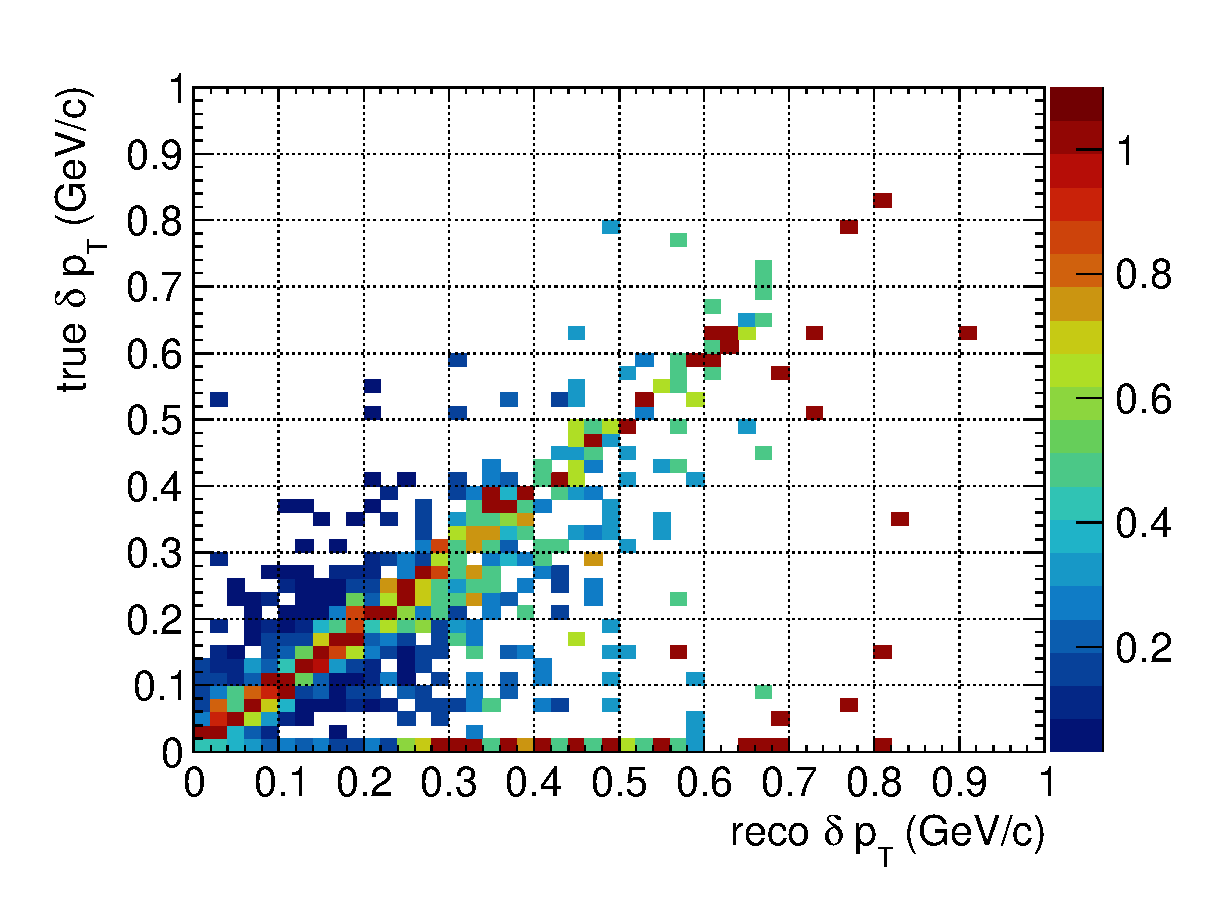
\includegraphics[width=\textwidth]{figures/perf/tki/dpt_colnor_resmat_al11_sfgmu.eps}
               \caption{$\dpt$ after ESC}
               \label{subfig:esc-dpt-afesc-sfgmu}
          \end{subfigure}
          \\
          \begin{subfigure}[b]{\dbfigwid\textwidth}
               \centering
               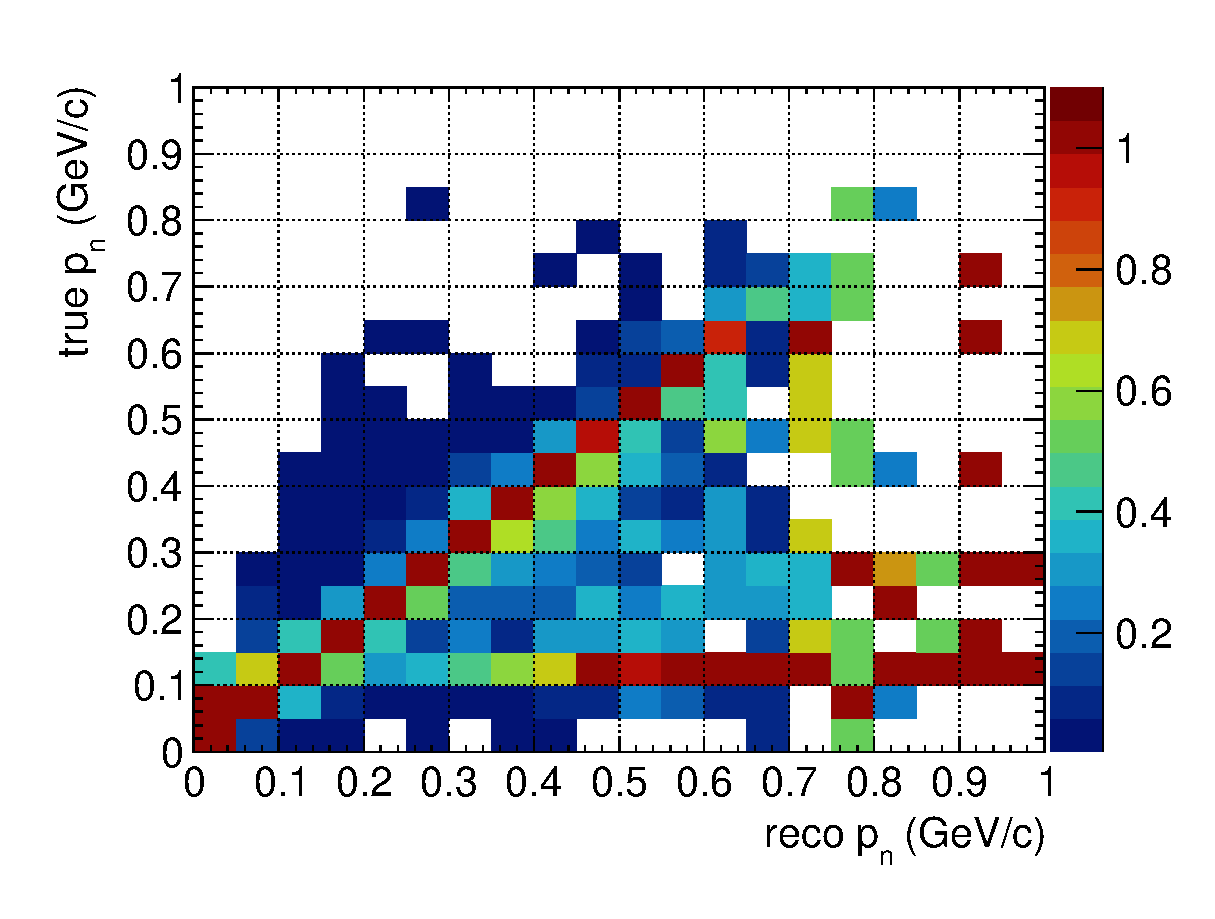
\includegraphics[width=\textwidth]{figures/perf/tki/pn_colnor_resmat_al10_sfgmu.eps}
               \caption{$\pn$ before ESC}
               \label{subfig:esc-pn-bfesc-sfgmu}
          \end{subfigure}
          \begin{subfigure}[b]{\dbfigwid\textwidth}
               \centering
               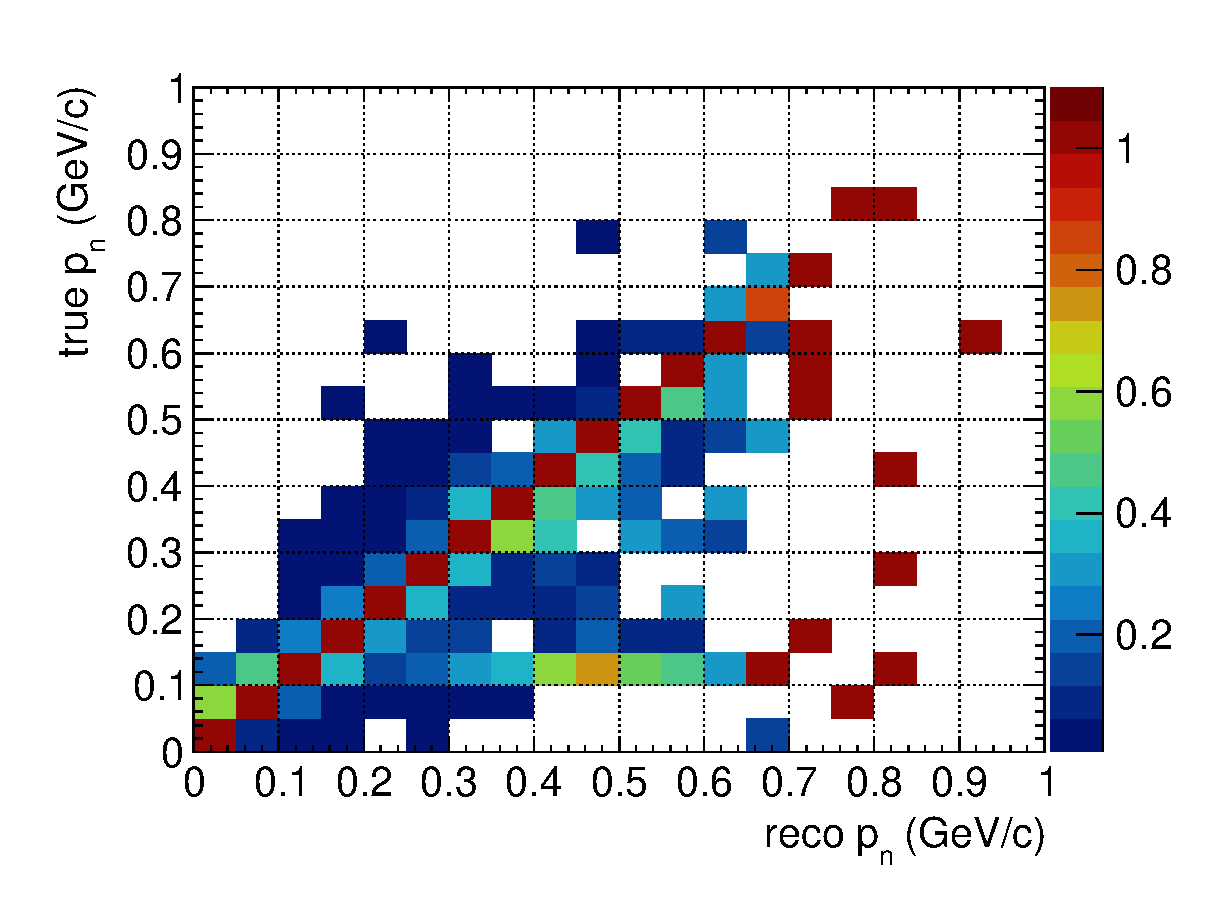
\includegraphics[width=\textwidth]{figures/perf/tki/pn_colnor_resmat_al11_sfgmu.eps}
               \caption{$\pn$ after ESC}
               \label{subfig:esc-pn-afesc-sfgmu}
          \end{subfigure}
          \caption{TKI variables before and after ESC for the $\numucczpiop$ selection for the SFGD-$\mu$ sub-sample.}
          \label{fig:mc-tki-0pi-esc-sfgmu}
     \end{figure}


     \begin{figure}
          \begin{subfigure}[b]{\dbfigwid\textwidth}
               \centering
               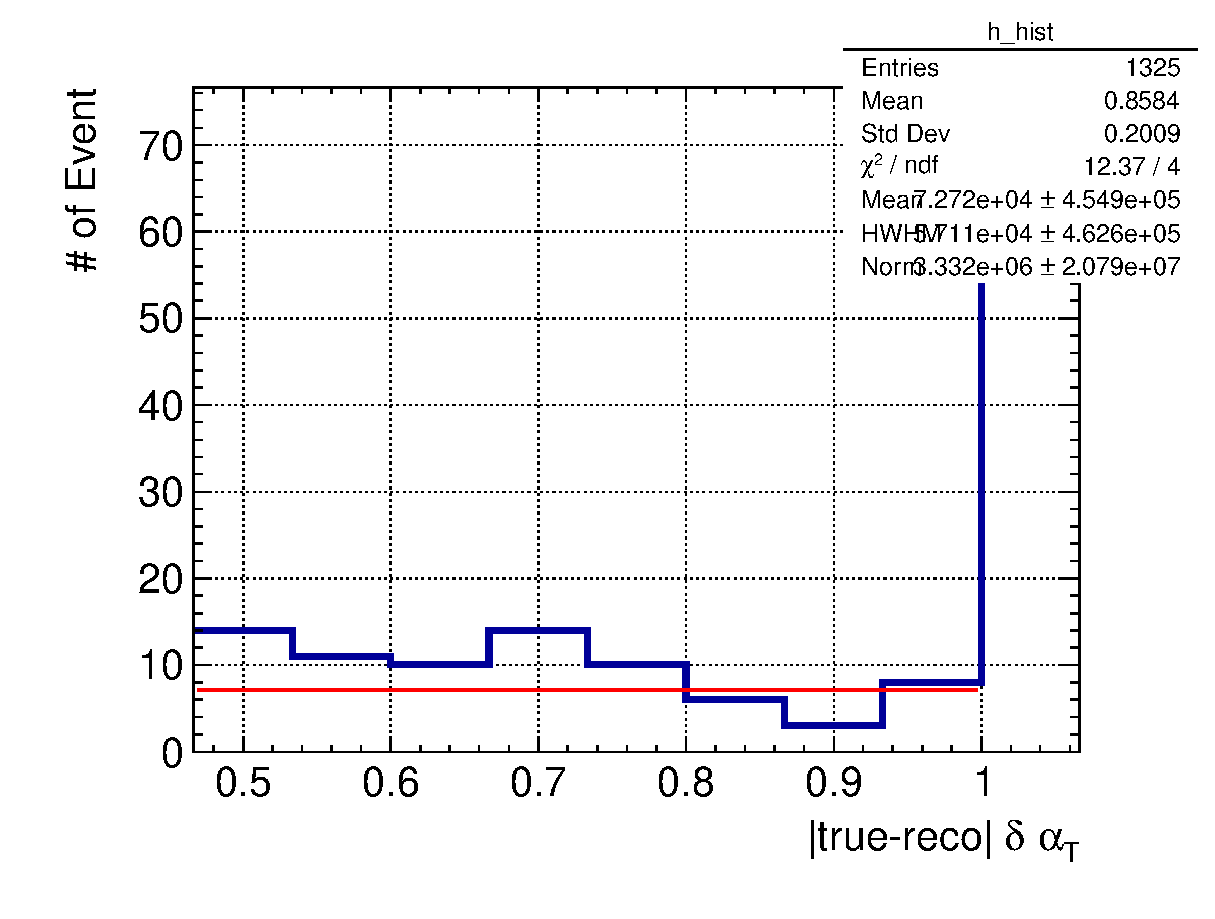
\includegraphics[width=\textwidth]{figures/perf/tki/dalphat_rat_hist_al11_sfgmu.eps}
               \caption{$\dat$ before muon bias correction}
               \label{subfig:esc-dalpha-bfmu-sfgmu}
          \end{subfigure}         
          \begin{subfigure}[b]{\dbfigwid\textwidth}
               \centering
               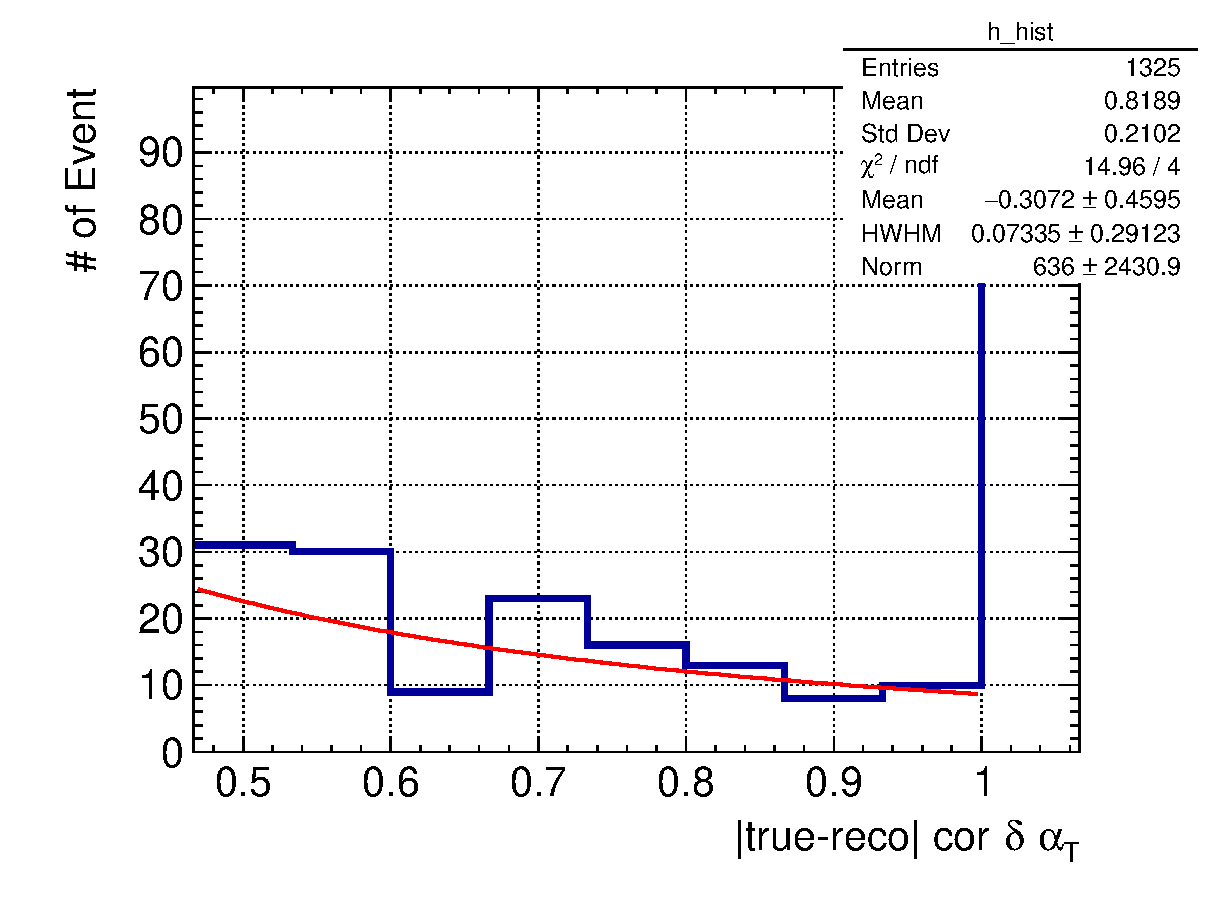
\includegraphics[width=\textwidth]{figures/perf/tki/cor_dalphat_rat_hist_al11_sfgmu.eps}
               \caption{$\dat$ after muon bias correction}
               \label{subfig:esc-dalpha-afmu-sfgmu}
          \end{subfigure}
          \\
          \begin{subfigure}[b]{\dbfigwid\textwidth}
               \centering
               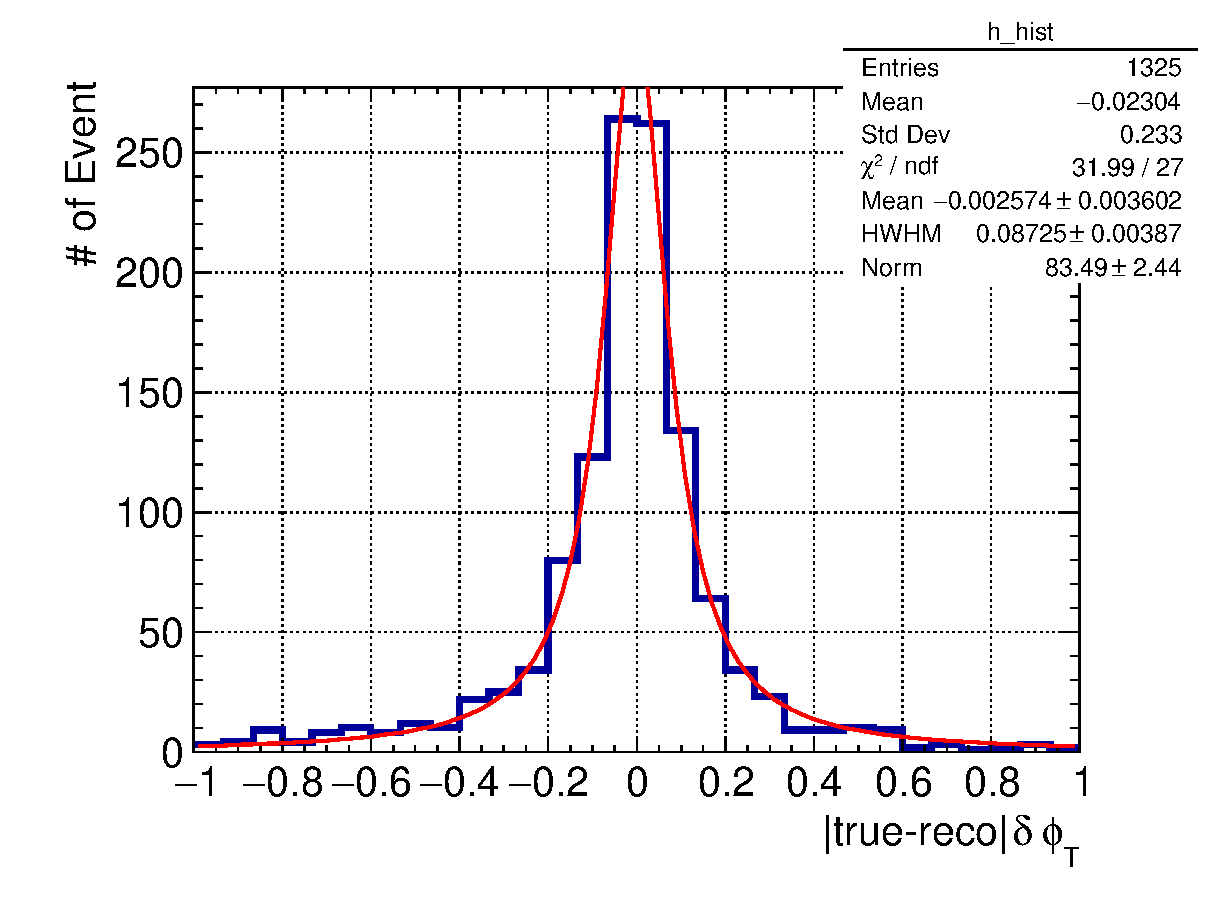
\includegraphics[width=\textwidth]{figures/perf/tki/dphit_rat_hist_al11_sfgmu.eps}
               \caption{$\dphit$ before muon bias correction}
               \label{subfig:esc-dphit-bfmu-sfgmu}
          \end{subfigure}
          \begin{subfigure}[b]{\dbfigwid\textwidth}
               \centering
               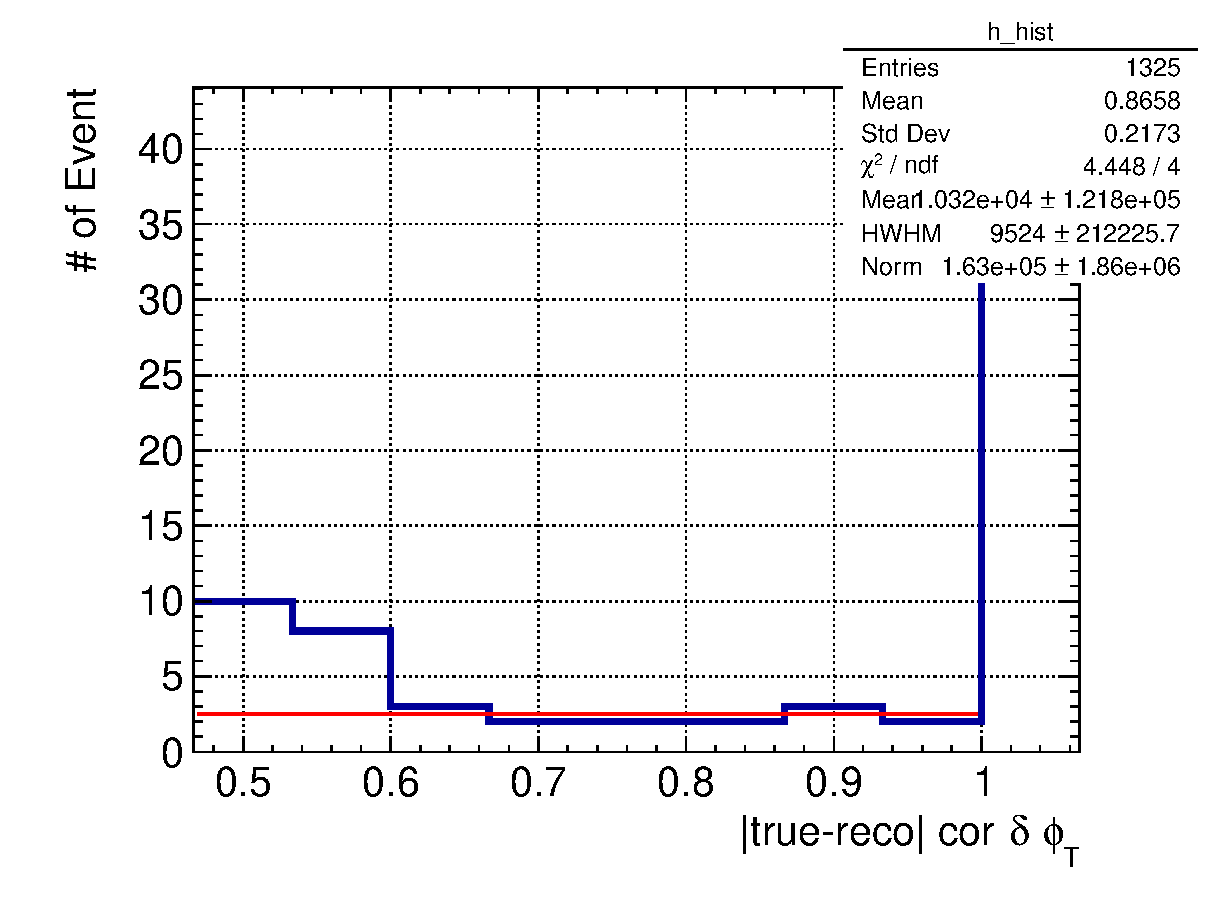
\includegraphics[width=\textwidth]{figures/perf/tki/cor_dphit_rat_hist_al11_sfgmu.eps}
               \caption{$\dphit$ after muon bias correction}
               \label{subfig:esc-dphit-afmu-sfgmu}
          \end{subfigure}
          \\
          \begin{subfigure}[b]{\dbfigwid\textwidth}
               \centering
               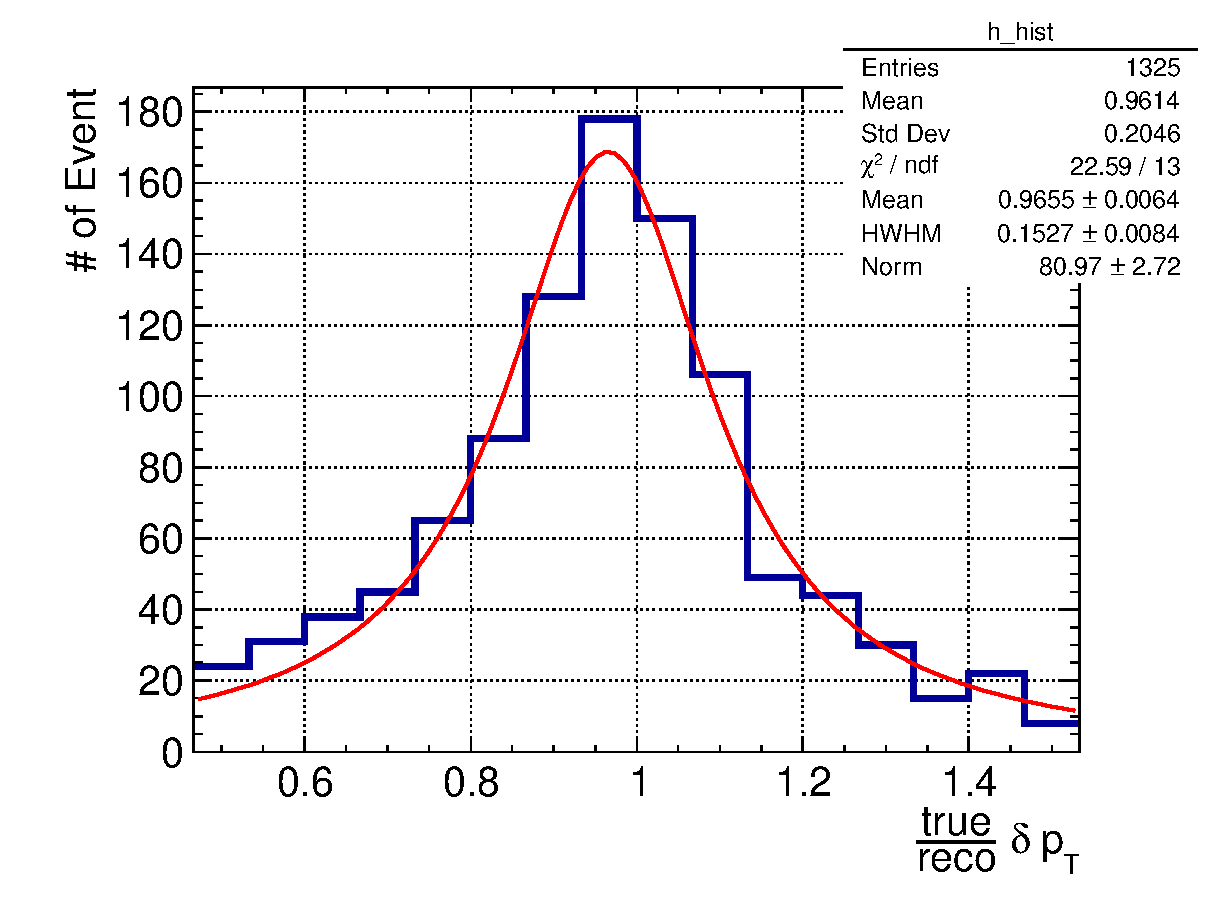
\includegraphics[width=\textwidth]{figures/perf/tki/dpt_rat_hist_al11_sfgmu.eps}
               \caption{$\dpt$ before muon bias correction}
               \label{subfig:esc-dpt-bfmu-sfgmu}
          \end{subfigure}
          \begin{subfigure}[b]{\dbfigwid\textwidth}
               \centering
               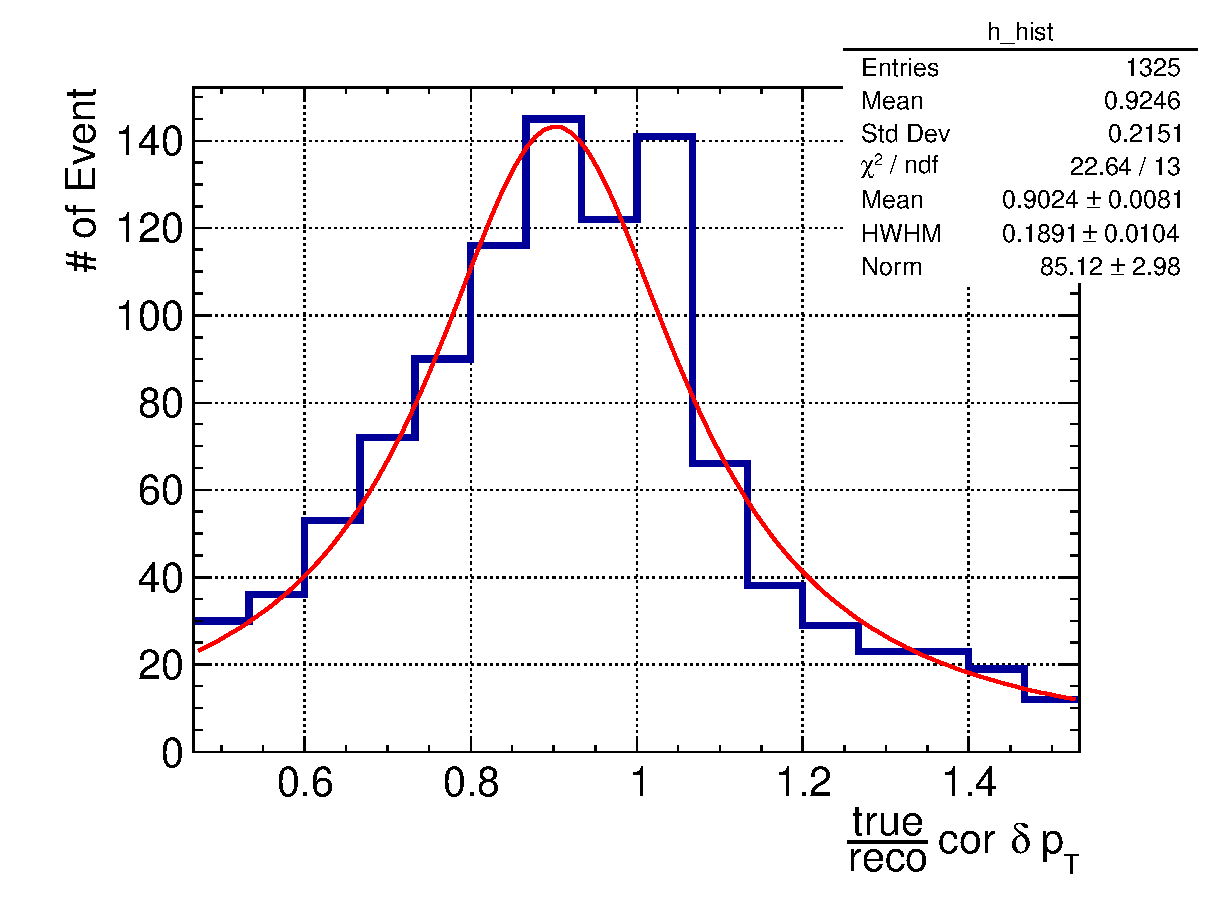
\includegraphics[width=\textwidth]{figures/perf/tki/cor_dpt_rat_hist_al11_sfgmu.eps}
               \caption{$\dpt$ after muon bias correction}
               \label{subfig:esc-dpt-afmu-sfgmu}
          \end{subfigure}
          \\
          \begin{subfigure}[b]{\dbfigwid\textwidth}
               \centering
               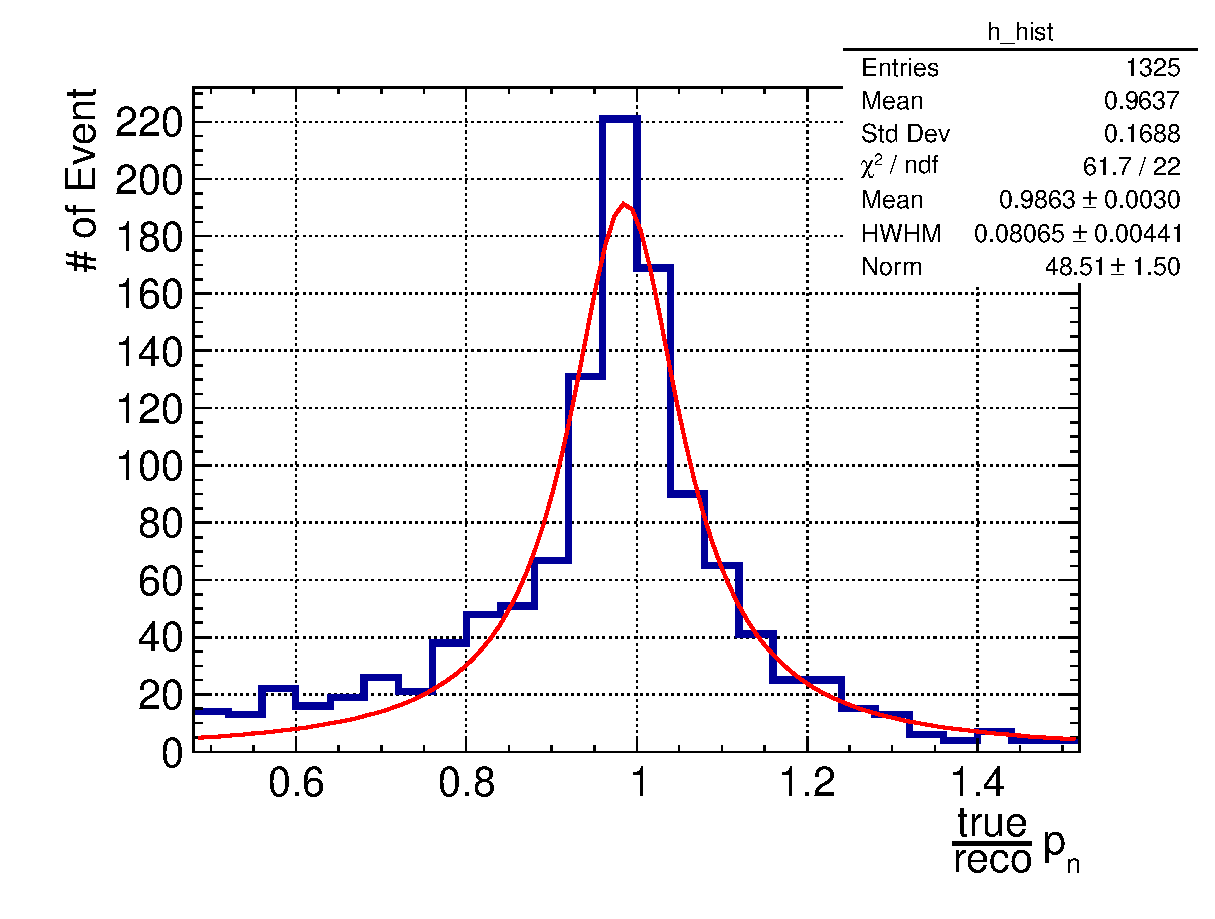
\includegraphics[width=\textwidth]{figures/perf/tki/pn_rat_hist_al11_sfgmu.eps}
               \caption{$\pn$ before muon bias correction}
               \label{subfig:esc-pn-bfmu-sfgmu}
          \end{subfigure}
          \begin{subfigure}[b]{\dbfigwid\textwidth}
               \centering
               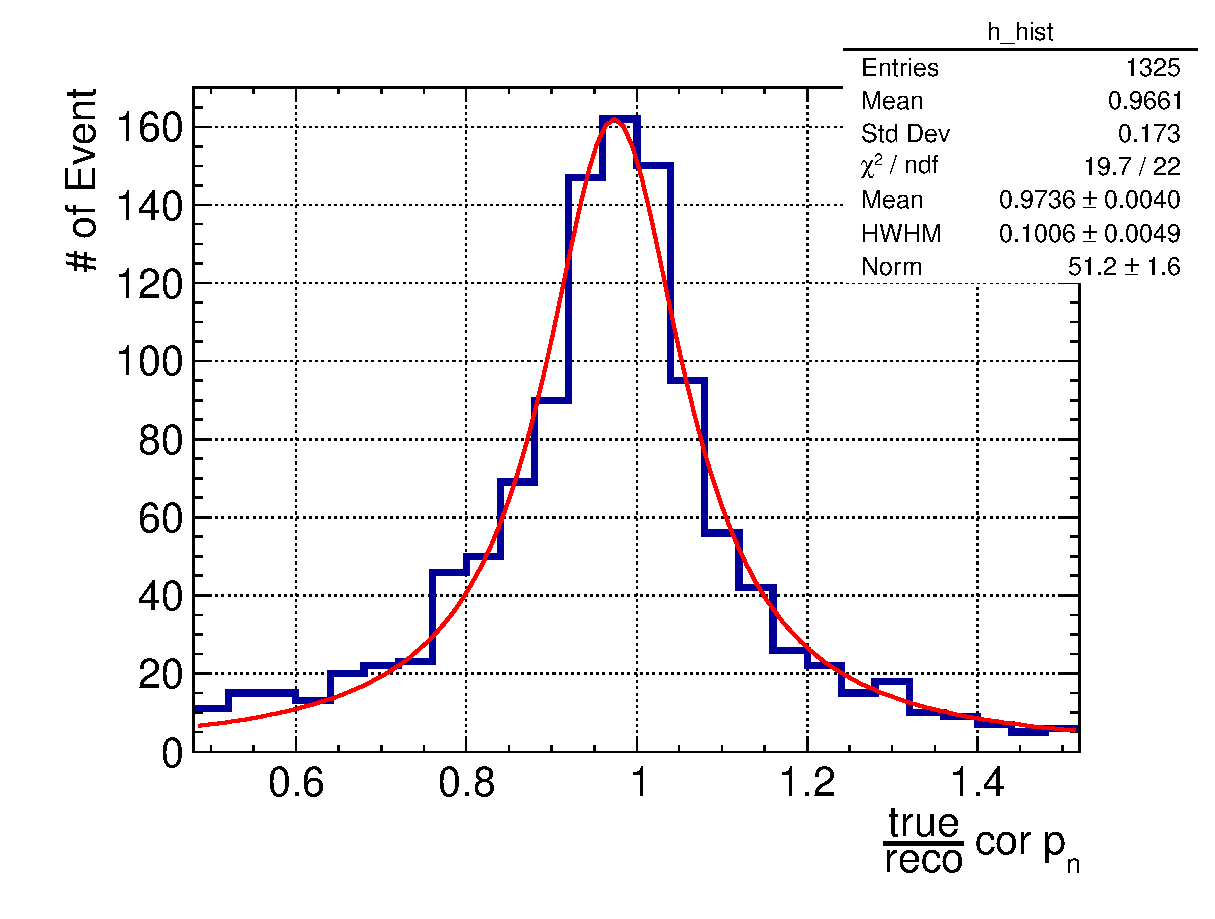
\includegraphics[width=\textwidth]{figures/perf/tki/cor_pn_rat_hist_al11_sfgmu.eps}
               \caption{$\pn$ after muon bias correction}
               \label{subfig:esc-pn-afmu-sfgmu}
          \end{subfigure}
          \caption{TKI variables before and after muon bias correction for the $\numucczpiop$ selection for the SFGD-$\mu$ sub-sample.}
          \label{fig:mc-tki-0pi-mu-sfgmu}
     \end{figure}
 